% This is a LaTeX thesis template for Monash University.
% to be used with Rmarkdown
% This template was produced by Rob Hyndman
% Version: 6 September 2016

\documentclass{monashthesis}

%%%%%%%%%%%%%%%%%%%%%%%%%%%%%%%%%%%%%%%%%%%%%%%%%%%%%%%%%%%%%%%
% Add any LaTeX packages and other preamble here if required
%%%%%%%%%%%%%%%%%%%%%%%%%%%%%%%%%%%%%%%%%%%%%%%%%%%%%%%%%%%%%%%

\author{Xiefei Li}
\title{Revisiting the Forecast Combination Puzzle: An Empirical Study}
\studentid{30204232}
\studentemail{\href{mailto:xlii0145@student.monash.edu}{\nolinkurl{xlii0145@student.monash.edu}}}
\studentdetails{Supervisor: David T. Frazier}
\supervisoremail{\href{mailto:David.Frazier@monash.edu}{\nolinkurl{David.Frazier@monash.edu}}}
\def\degreetitle{Bachelor of Commerce (Honours)}
% Add subject and keywords below
\hypersetup{
     %pdfsubject={The Subject},
     %pdfkeywords={Some Keywords},
     pdfauthor={Xiefei Li},
     pdftitle={Revisiting the Forecast Combination Puzzle: An Empirical Study},
     pdfproducer={Bookdown with LaTeX}
}


\bibliography{thesisrefs}

\begin{document}

\pagenumbering{roman}

\titlepage

{\setstretch{1.2}\sf\tighttoc\doublespacing}

\clearpage\pagenumbering{arabic}\setcounter{page}{1}

\hypertarget{abstract}{%
\chapter*{Abstract}\label{abstract}}
\addcontentsline{toc}{chapter}{Abstract}

This thesis demonstrates that the forecast combination puzzle is tightly related to the in-sample fit of constituent models used in the analysis. The forecast combination puzzle refers to the common finding that an equally-weighted forecast combination often outperforms an optimally-weighted forecast combination calculated via a sophisticated scheme. We show that when constituent models have similar in-sample fit, the puzzle will be in evidence; it is ambiguous otherwise. We analytically show the relationship between the estimated optimal weight and the constituent models in terms of point combinations using mean squared error and empirically confirm these findings in density combinations using log score. As an additional contribution, the puzzle is shown to be evident in both time series and cross-sectional settings.

\vspace{1cm}

\textit{Keywords}: Forecast Combination, Forecast Combination Puzzle, Point Forecasting, Probabilistic Forecasting, Scoring Rules

\newpage

\hypertarget{acknowledgements}{%
\chapter*{Acknowledgements}\label{acknowledgements}}
\addcontentsline{toc}{chapter}{Acknowledgements}

I would like to express my deepest appreciation to my supervisor David Frazier and my Honours coordinator Heather Anderson for their incredibly valuable guidance, feedback and patience. I am also grateful to receive the Econometrics Honours Memorial Scholarship from Monash University to support my Honours study. Special thanks to my parents, my friends and those people who gave me advice and helped me throughout the year.

\hypertarget{introduction}{%
\chapter{Introduction}\label{introduction}}

\hypertarget{research-objective}{%
\section{Research Objective}\label{research-objective}}

This thesis aims to investigate the determinants behind, and evidence for the forecast combination puzzle in various domains. The combination puzzle refers to the well-known empirical finding that an equally weighted combination of forecasts generally outperforms more sophisticated combination schemes. While this phenomenon is often referenced in the point forecast combinations literature, it is also present in the literature on density forecast combinations. Starting with two different types of time series datasets, several two-model pools are constructed to explore how the presence of the puzzle relates to the in-sample performance of the constituent models used to produce the combination.

The empirical studies undertaken so far have focused more on pure time series settings, while there is little literature on the puzzle in the cross-sectional setting. A simulated study is designed to investigate the puzzle in the two-model pool under a regression analysis. In addition, we derive and obtain a closed-form expression that supports this finding in the linear regression case. Throughout, we measure the performance of density combinations via the log score function and use mean squared forecast error to assess the accuracy of point combinations.

\hypertarget{literature-review-and-motivation}{%
\section{Literature Review and Motivation}\label{literature-review-and-motivation}}

Forecast accuracy is of critical concern to forecasters and decision makers. The application of forecast combination, originally proposed in the seminal work of \textcite{BG69}, provides improvements in forecast accuracy relative to individual forecasts, and therefore has attracted wide attention and contributions in the literature, both theoretical and applied \autocite{C89,T06}. More importantly, this approach often has robust performance across various types of data, proved by numerous empirical results \autocite{GA11}. Many researchers also devote efforts on probabilistic forecasting to obtain more information about the uncertainty of the resulting forecast. Similar to point forecasts, researchers have found that density forecast combination outperform individual density forecast \autocites[e.g.,][]{HM07,GA11}.

Forecast combination methods, in general, involve combining multiple forecasts generated from individual or constituent models based on a rule or weighting scheme. Every scheme has its own objective function for producing the ``best'' forecast combination, along with the optimal weight assigned to each model. This process can sometimes capture more meaningful characteristics of the true data generating process than using a single model, and allows us to combine the best features of different models within a single framework. Researchers have examined a variety of combination methods for both point and density forecasts over the past 50 years, see \textcite{WHLK22} for a modern literature review.

In most time series setting under which forecast combinations are employed, a striking empirical phenomenon is often observed, coined by \textcite{SW04}, as the ``forecast combination puzzle''. The puzzle is encapsulated by the fact that ``theoretically sophisticated weighting schemes should provide more benefits than the simple average from forecast combination, while empirically the simple average has been continuously found to dominate more complicated approaches to combining forecasts'' \autocite{WHLK22}. In other words, complex weighting schemes designed to improve in-sample accuracy should in theory perform better out-of-sample. However, the mean of the constituent forecasts appears to be more robust in practice than forecasts combined through complicated weighting schemes. This finding has been continuously reaffirmed by extensive literature reviews and papers \autocites[e.g.,][]{MACF82,C89,MSA18,MSA20}, and the simple averaging naturally becomes a benchmark. For the purposes of this analysis, we explicitly define the forecast combination puzzle as: 1) the simple average has better out-of-sample performance than that of the optimal combination; and 2) the forecast accuracy between the optimal combination and the simple average being small, which allows for the optimal combination to be slightly higher than the simple average. As the forecast accuracy is not too different, using either combination method will not make a meaningful difference, except in special circumstances.

The literature explains the puzzle mainly in three aspects: the estimation uncertainty in complicated weighting schemes \autocite{SW98,SW04,SW09}, the bias and inefficiency in the Mean Squared Forecast Error (MSFE) function \autocite{E11,CMVW16}, and the sampling variability of the forecasts induced via estimation of the constituent model forecasts \autocite{ZMFP22,FZMP23}. However, all of these explanations implicitly assume that the puzzle will be in evidence when combining forecasts, regardless of the choice of constituent models or the weighing scheme. They overlook the possibility that complicated combination methods can perform better than the simple average in some cases. In order to make a rigorous explanation statement, we systematically explore the determinants behind the presence of the puzzle. Even though there is a widespread literature among different pure time series settings, no attention appears to have been given to the cross-sectional setting. Therefore, we will investigate the puzzle in both time series and cross-sectional settings using empirical and simulated data respectively.

Considering a simple case of two-model combination, our initial conjecture is that the presence of the puzzle is tightly-related to the in-sample fit of two constituent models. We conjecture that when constituent models have similar in-sample fit, the puzzle will be in evidence. Otherwise, the presence of the puzzle is uncertain. Intuitively, the model in-sample performance greatly affects the behavior of forecasts, so forecasts produced by two similarly performed models will not differ much, leading to an estimated optimal weight around a half. Consequently, we should expect small differences in forecast accuracy between optimally-combined forecast and equally-combined forecast. It is then reasonable to prefer the simple average given that the forecast variance will also be lessened due to no extra parameter estimation. On the contrary, if two models have distinct in-sample fit, we conjecture that the optimal forecast combination will give more weight to the better performing forecast and therefore the estimated weights will be far away from a half. The estimated value of the optimal weight does not indicate the forecast accuracy of the optimal forecast combination. Therefore, there are two possible situations: the equally-combined forecast perform better than the optimally-combined forecast, and the opposite. The presence of the puzzle now becomes ambiguous, depending on the situation we fall into. According to the definition of the puzzle, our conjecture can be summarized in Table \ref{tab:1}. Two constituent models are evaluated based on their in-sample relative performance and are also allowed to perform equivalently \texttt{Bad} for different reasons.

\begin{table}[ht]
\centering
\begin{tabular}{cccc}
                       &      & \multicolumn{2}{c}{$M_2$} \\
                       &      & Good       & Bad       \\
\multirow{2}{*}{$M_1$} & Good & $\surd$    & $?$ \\
                       & Bad  & $?$        & $\surd$
\end{tabular}
\caption{The first row and the first column refer to two constituent models in a combination, $M_1$ and $M_2$. ``Good`` means that the model fits the data well, whereas ``Bad`` denotes that the model fails to capture some important features of the data. The ``$\surd$`` indicates the presence of the forecast combination puzzle, while ``$?$`` implies that the presence of the puzzle is uncertain.}
\label{tab:1}
\end{table}

We demonstrate that the forecast combination puzzle is in evidence in the time series setting with the S\&P500 index and the quarterly unemployment data. That is, the equally-weighted combination provides equivalent or superior forecast accuracy relative to the optimally-weighted combination. We then compare the in-sample fit of constituent models using their in-sample log likelihood and validate most of our conjecture.

Furthermore, we investigate the forecasting performance of two-model pools for simulated cross-sectional data using simple linear regression models. We derive a mathematical relationship between the optimal combination weight under the mean squared forecast error and elements in the true DGP. This relationship implies that the forecast combination puzzle is tightly-related to the interaction between constituent models and the true DGP. Given this knowledge in the point combination setting, we empirically investigate this finding for density combinations and validate that these formal reasoning are applicable in a more general setting. In addition, this simulation study provides sufficient empirical evidence to examine conjecture.

The goal of this thesis is two-fold: first, to substantiate the presence of the combination puzzle in the time series setting and to explore the relationship between the puzzle and the in-sample fit of constituent models; second, to mathematically derive the formula of the optimal weight in the regression setting under mean squared forecast error and then to validate the conjecture in Table \ref{tab:1} with empirical evidence.

The thesis follows two common weighting schemes for \texttt{two\ model} pools (Section 2) and then applies the log score to density combinations for daily S\&P 500 index and the mean squared error to point combinations for quarterly number of unemployed (Section 3). With some empirical evidence of the conjecture, Section 4 derives a closed-form expression for the optimal weight under the mean squared error in a simple regression case. The findings are further examined by analyzing density combinations in the cross-sectional setting. The final section concludes.

\hypertarget{method}{%
\chapter{Methodology}\label{method}}

In the literature, there are several definitions of combinations. We focus on the combination of forecasts from non-nested models for a given dataset, which is commonly performed in two stages:

\begin{enumerate}
\def\labelenumi{\arabic{enumi}.}
\item
  producing separate point or probabilistic forecasts for the next time point using observed data and constituent models;
\item
  combining forecasts based on a given accuracy criteria.
\end{enumerate}

We only consider the combination of two individual forecasts, i.e., two constituent models, to simplify the analysis through fast and relative simple data manipulation.

Before explaining details, the following notation will be used throughout the paper. To examine forecast accuracy, we partition on observed time series \(y_t\) with a total of \(T\) observations into two proportional parts, an in-sample period with \(R\) observations and an out-of-sample period with \(P\) observations. We restrict the analysis to a 1-step ahead prediction, conditioning on the information set at time t, \(\mathcal{F}_t\), which is comprised of all observed (and known) realizations of \(y\) up to time t, i.e., \(\mathcal{F}_t = \{y_1, y_2, .., y_t\}\).

Every proposed parametric model determines the conditional probability density for \(y_t\), denoted by \(f(y_t|\mathcal{F}_{t-1}, \theta)\), given unknown parameters \(\theta\) and all the past information \(\mathcal{F}_{t-1}\). The choice and specification of constituent models vary by the features of the in-sample data. For each model, the maximum likelihood estimation method is applied to generate the estimators of unknown parameters, i.e., \(\hat\theta = \underset{\theta \in \Theta}{\arg\max} \sum^R_{t=1} log f(y_t|\mathcal{F}_{t-1}, \theta)\). Given the log likelihood function of in-sample period for each model, the corresponding estimates are obtained when they maximize that function and then held fixed for out-of-sample procedures. The optimal combination is then constructed with the estimated weight of each model that delivers the best in-sample accuracy.

\hypertarget{density-combinations}{%
\section{Density combinations}\label{density-combinations}}

\subsection*{Linear pooling}

Consider the case of two competing models, which we identify through their probability densities. Undoubtedly, densities can be combined in many ways; see Section 3 of \textcite{WHLK22} for many popular means of probabilistic combination. One of the commonly used approaches is the ``linear opinion pool'', which weights densities in a linear form \autocites[e.g.,][]{BG69,HM07,GA11}. For two-model pools, constituent densities \(f_1(y_t)\) and \(f_2(y_t)\) are combined as follows:
\begin{equation*}
f_{\omega}(y_t) = \omega \ f_1(y_t | \mathcal{F}_{t-1}, \theta_{1}) + (1-\omega) f_2(y_t | \mathcal{F}_{t-1}, \theta_{2}),
\end{equation*}
where \(\omega \in [0,1]\) is the non-negative weight allocated to the probability density attributed to the first model. Two densities are often determined by different sets of parameters, differentiated by \(\theta_{1}\) and \(\theta_{2}\). Through this construction, the sum of the model weights is fixed at 1, which is a necessary and sufficient condition for \(f_{\omega}(y_t)\) to be a proper density function \autocite{GA11}. In addition to producing point forecasts, density forecasts can offer forecasters or decision markers a comprehensive view of the target variable (see section 2.6.1. of \textcite{FTP22} for related contributions).

\vspace{5mm}

\subsection*{Log scoring rules}

Following the literature on density evaluation, our initial analysis will focus on using log score to measure the accuracy of our density forecasts; see, e.g., \textcite{GA11} for a discussion on log score and its use in density forecasting. For each individual model, the log score over the in-sample period is:\\
\begin{equation*}
LS = \sum^R_{t=1} log \ \hat f(y_t| \mathcal{F}_{t-1}, \hat\theta).
\end{equation*}

The optimal linear combination is identified to produce the most accurate forecasts when the set of weights maximizes the log score function of two densities over the in-sample \(R\) observations,
\begin{equation}
\label{eqn:LS2}
\hat{\omega}_{\text{opt}} =  \underset{\omega \in [0,1]}{\arg\max} \sum^R_{t=1} log \Big[ \omega \ \hat f_1(y_t| \mathcal{F}_{t-1}, \hat\theta_{1}) + (1-\omega) \ \hat f_2(y_t| \mathcal{F}_{t-1}, \hat\theta_{2})\Big].
\end{equation}

Thus, the log predictive score over the out-of-sample period \(t = R+1, R+2, \dots, T\) is:
\begin{equation}
\label{eqn:LS3}
LPS = \sum^T_{t = R+1} log \Big[ \hat{\omega}_{\text{opt}} \ \hat f_1(y_t| \mathcal{F}_{t-1}, \hat\theta_{1}) + (1- \hat{\omega}_{\text{opt}}) \ \hat f_2(y_t| \mathcal{F}_{t-1}, \hat\theta_{2})\Big].
\end{equation}

\hypertarget{point-combinations}{%
\section{Point combinations}\label{point-combinations}}

Although our main focus is density forecast combination, to simplify certain analysis, point forecast combination is also considered The point forecast of each model corresponds to the mean value of the predictive density. We use mean squared forecast error (MSFE), following \textcite{BG69} and \textcite{SW09}, to measure the accuracy of point forecasts in the two-model pools.

\subsection*{Linear combination}

Similar to the density case, points from two constituent models, \(y_{1t}\) and \(y_{2t}\), are aggregated linearly:
\begin{equation*}
y_t({\omega}) = \omega \ y_{1t} + (1-\omega) \ y_{2t},
\end{equation*}
where \(\omega\in [0,1]\) is the non-negative weight allocated to the point forecast generated from the first model.

\vspace{5mm}

\subsection*{Mean squared forecast error}

The mean squared error (MSE) of the individual prediction is the average squared difference between the actual value, \(y_t\), and the predicted value, \(\hat y_t\), at each time point over the in-sample period:

\begin{equation*}
MSE = \frac{1}{R} \sum^R_{t=1} (y_t - \hat y_t)^2.
\end{equation*}

The lower the MSE, the higher the accuracy of the forecast. Therefore, the ``optimal'' set of weights minimizes the MSE of the point forecast combination among all other possible sets over the \(R\) in-sample observations:
\begin{equation*}
\hat{\omega}_{\text{opt}} = \underset{\omega \in [0,1]}{\arg\min} \frac{1}{R} \sum^R_{t=1} \Big[y_t - (\omega \ \hat y_{1t} + (1-\omega) \ \hat y_{2t})\Big]^2.
\end{equation*}

Consequently, the MSFE over the out-of-sample period \(t = R+1, R+2, \dots, T\) is:
\begin{equation*}
MSFE = \frac{1}{P} \sum^T_{t = R+1} \Big[y_t - (\hat{\omega}_{\text{opt}} \ \hat y_{1t} + (1-\hat{\omega}_{\text{opt}}) \ \hat y_{2t}) \Big]^2.
\end{equation*}

\hypertarget{empirical-results}{%
\chapter{Empirical Results}\label{empirical-results}}

\hypertarget{sp500}{%
\section{Daily time series (S\&P 500)}\label{sp500}}

Reconsidering the example in Section 3 of \textcite{GA11}, the data we use is the daily Standard and Poor's (S\&P) 500 index from February 11, 2013 to February 10, 2023 (10 years in total), retrieved from Federal Reserve Economic Data \autocite{SP500}. The S\&P 500 index dataset has \(T = 2519\) total observations and is partitioned into two periods with a rough proportion. The in-sample period contains the first 60\% of the data (\(R = 1511\)), which is used to estimate all unknown parameters, including the optimal weight. The remaining 40\% (\(P = 1008\)) is reserved to evaluate forecast performance.

We will investigate the presence of the forecast combination puzzle when both models fit the training set well and when one model badly fits the data. Three predictive models are chosen to study the performance of density predictions across sets of two-model pools from common classes of linear time series models: autoregressive integrated moving average (ARIMA), exponential smoothing (ETS), and linear regression model with ARIMA errors (LR). Detailed model specifications are elaborated in the Appendix.

We use \(P(A_1, A_2; \omega_{opt})\) to denote a two-model pool, where \(A_1\) and \(A_2\) are constituent models in the pool and \(\omega_{opt}\) is the optimal weight assigned to the first model \(A_1\).

\subsection*{Nonstationary time series}

To reduce the level of variability, we take a natural logarithm of the S\&P 500 index. Three candidate models are proposed to fit the log of the index, resulting in three sets of two-model combinations in total. The weight \(\omega\) takes values on a grid from 0 to 1 with increment of 0.01. The log score, as a function of the weight \(\omega\), is generated to search for the optimal weight over the in-sample period (refer to the top row of Figure \ref{fig:nonstat}). According to equation (\ref{eqn:LS2}), the estimated optimal weight corresponds to the maximum point of the curve. Then we can calculate the log predictive score of the optimal combination for the out-of-sample period based on equation (\ref{eqn:LS3}).

\begin{figure}[ht]
\centering
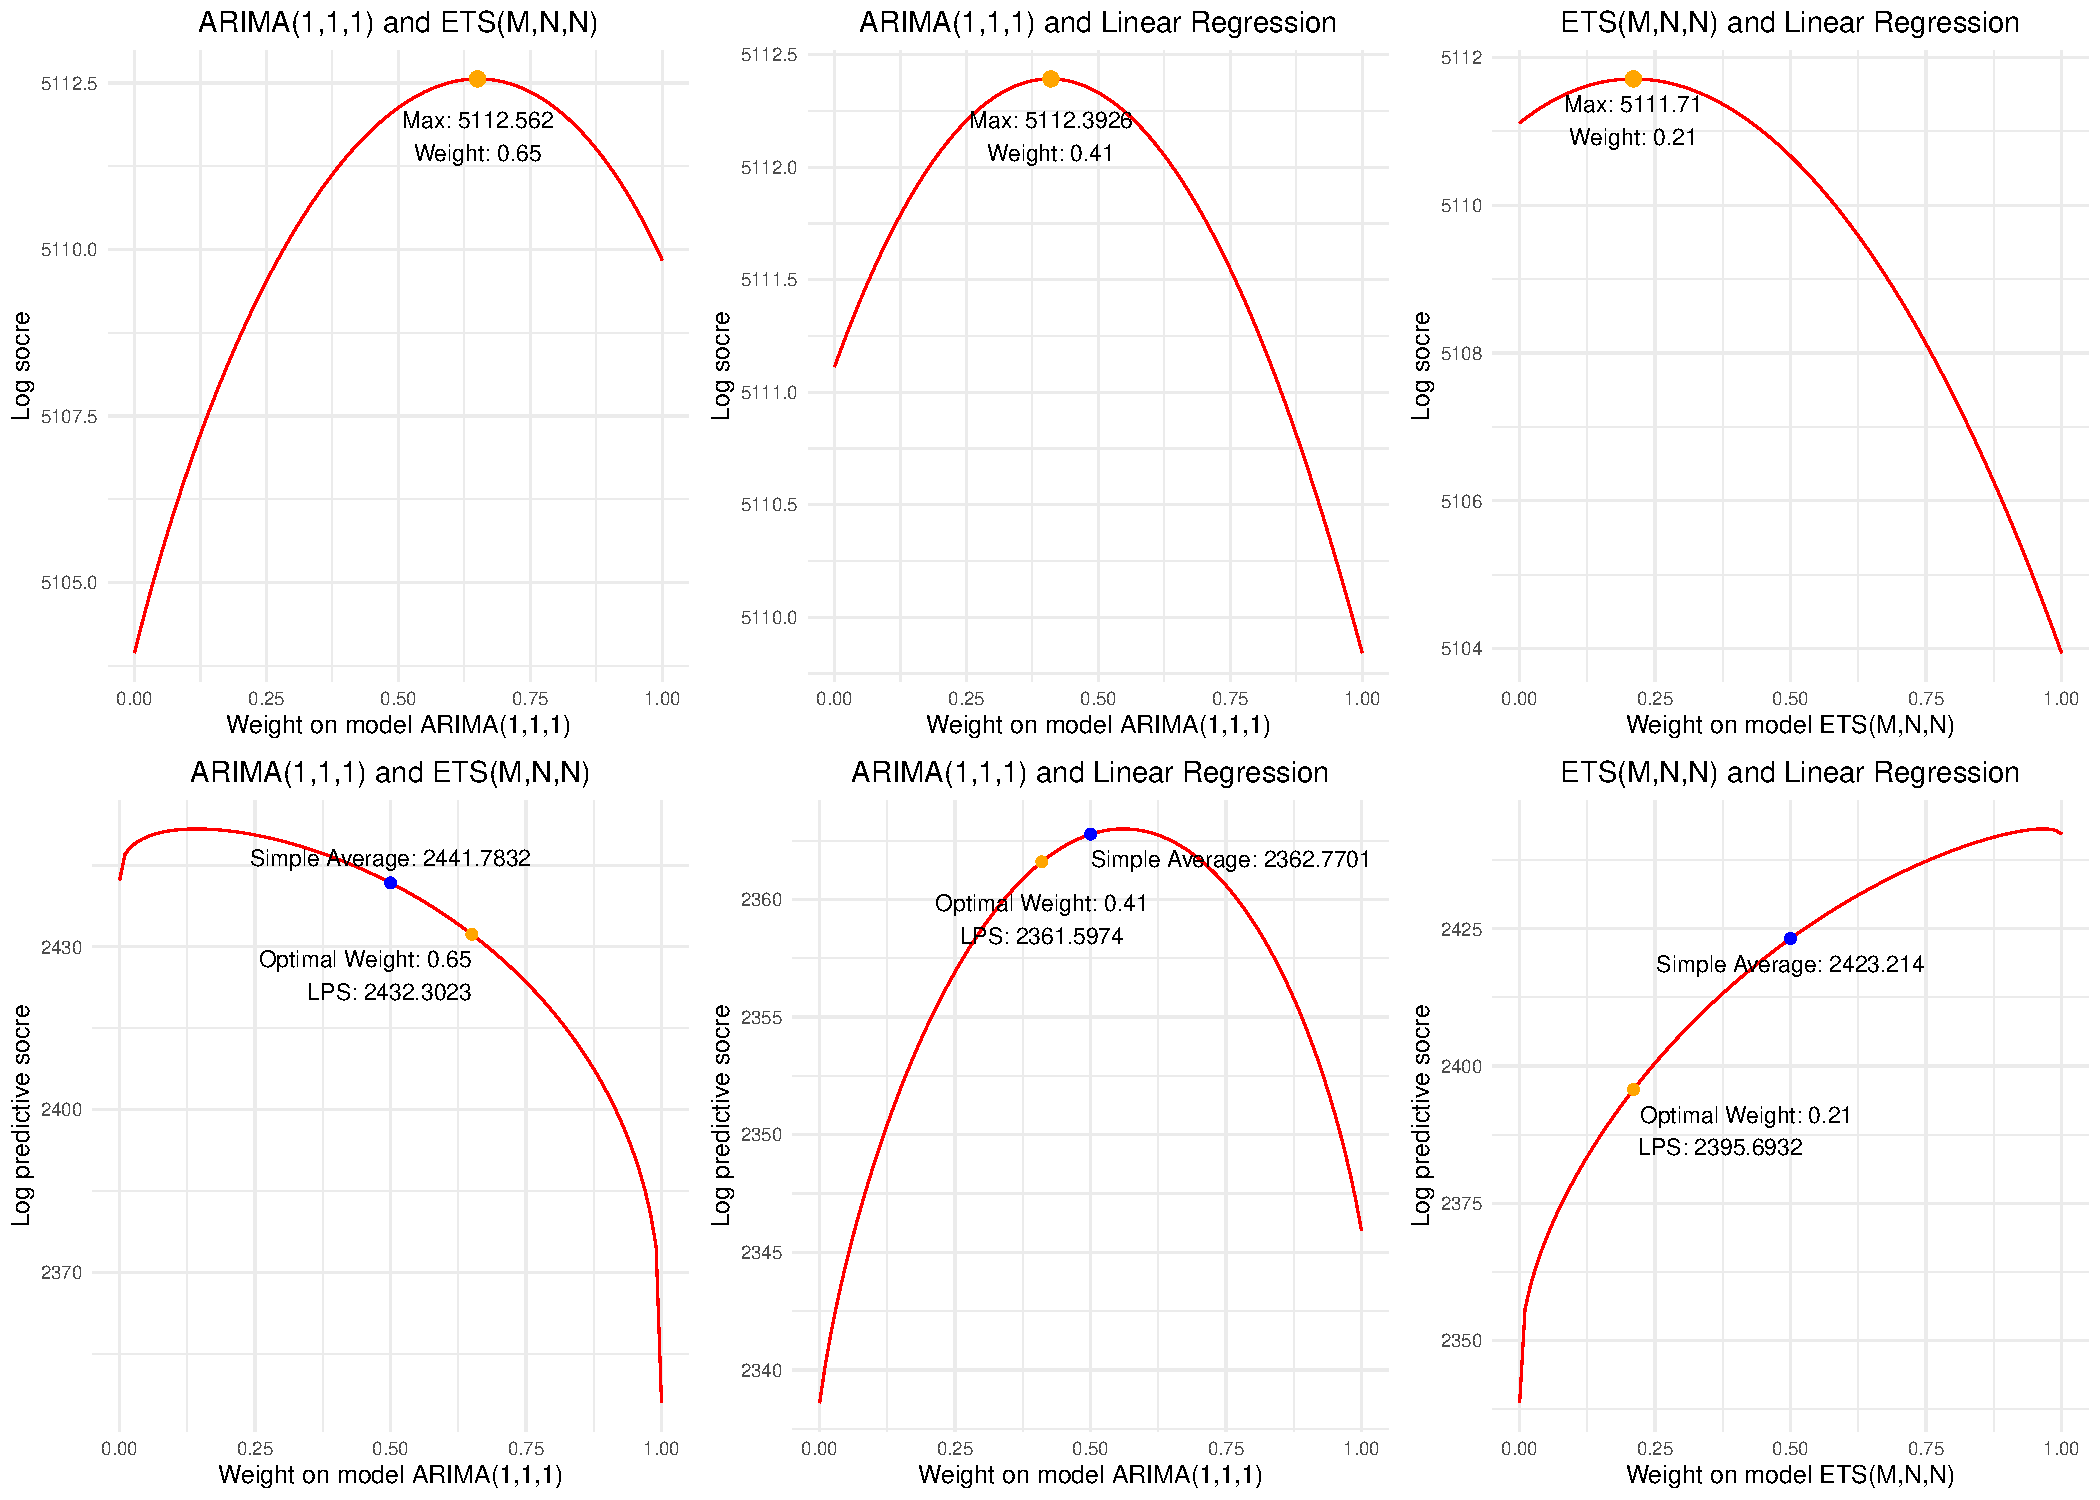
\includegraphics[scale=0.45]{figures/SP500_nonstationary.pdf}
\caption{Log predictive score of S\&P 500 index predictive densities in two-model pools over the in-sample (top) and out-of-sample (bottom) period. Constituent prediction models are described in the title with `P` representing `Pool`. The x-axis represents the weight assigned on the former model of the combination and the y-axis indicates the log predictive score. The orange dot represents the optimal combination, while the blue dot indicates the simple average.}
\label{fig:nonstat}
\end{figure}

Figure \ref{fig:nonstat} suggests that the forecast combination puzzle is evidenced in all three cases, i.e., the simple average performs better than the optimal combination. It is noticeable that the accuracy differences are different. For example, the accuracy difference in P(ARIMA,LR; 0.41) is much smaller than that in other two pools. This is tightly related to the in-sample fit of the constituent models, which can be represented by the log likelihood value. Table \ref{tab:nonfit} illustrates the log likelihood values of constituent models in each pool and the absolute difference.

One explanation for the poor performance of the ETS(M,N,N) model could be that it fails to capture the trend component, as shown in Figure \ref{fig:llg}. Compared with ARIMA and linear regression, the ETS model fits the training set poorly, making it a relatively \texttt{Bad} model in two-model pools as a consequence.

\begin{figure}[ht]
\centering
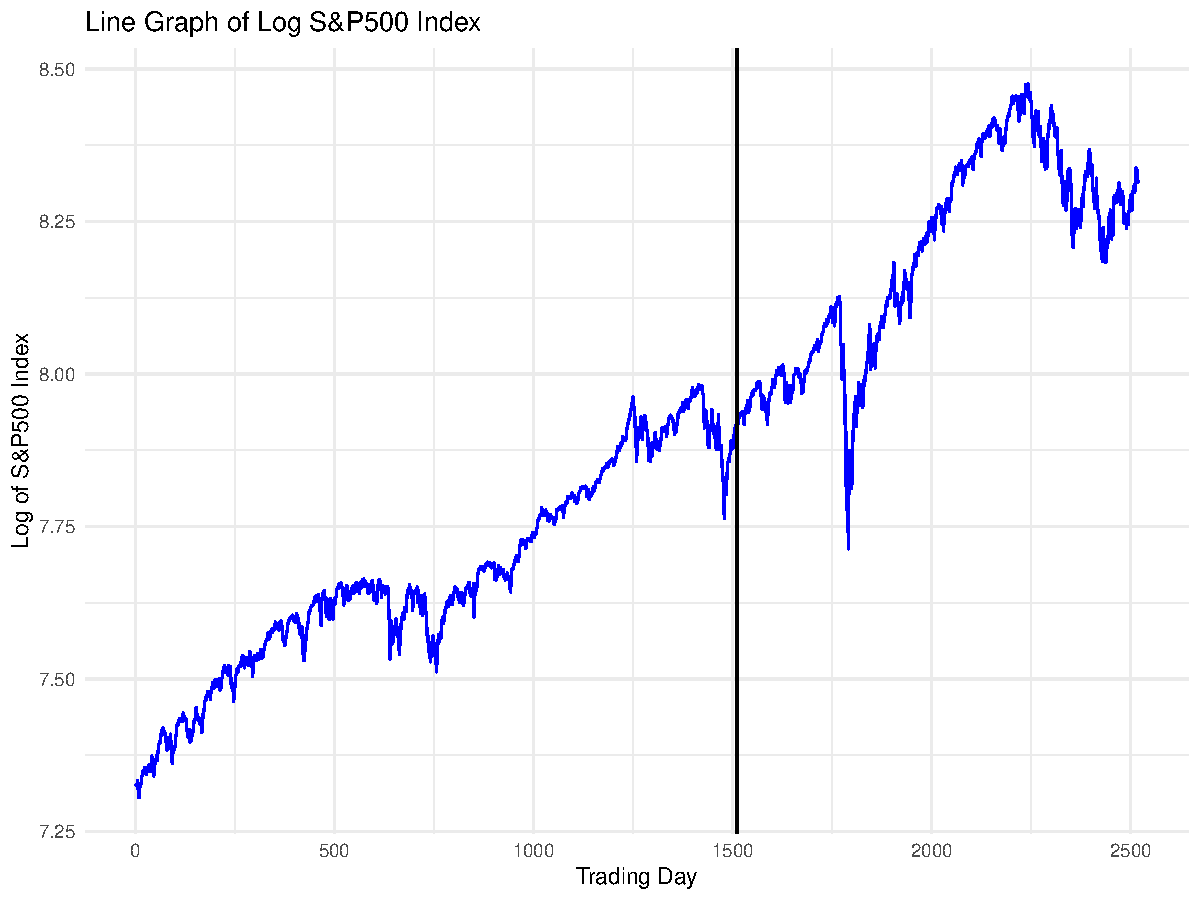
\includegraphics[scale=0.5]{figures/log_linegraph.pdf}
\caption{The black vertical line separates the traning set and the evaluation set. The training set is on the left and the evaluation set is on the right.}
\label{fig:llg}
\end{figure}

Linking it with our preliminary conjecture in Table \ref{tab:1}, P(ARIMA,ETS; 0.65) can be viewed as a (B,G) case where the ARIMA model has a much better in-sample fit than the ETS mode. Similarly, we have a (G,B) case for P(ETS,LR; 0.21) since the LR model performs much better than the ETS model. P(ARIMA,LR; 0.41), on the other hand, exemplifies a (G,G) case since two models fit the in-sample data well.

\begin{table}[ht]
  \centering
    \begin{tabular}{l|ccc}
    \toprule
                                    & P(ARIMA,ETS; 0.65) & P(ARIMA,LR; 0.41) & P(ETS,LR; 0.21) \\  
    \midrule
    First Model Log Likelihood      &     5113.694       &      5113.694     &   1725.137      \\
    Second Model Log Likelihood     &     1725.137       &      5116.014     &   5116.014      \\
    Log Likelihood Difference       &     3388.556       &       2.320       &   3390.876      \\
    Type                            &       (G,B)        &       (G,G)       &     (B,G)       \\
    Presence of the puzzle          &       Yes          &        Yes        &     Yes         \\
    \bottomrule
    \end{tabular}
  \caption{``Log Likelihood Difference`` represents the absolute difference of in-sample fit between two models, which is evaluated by the log likelihood. ``Type`` refers to the case of each two-model pool in the conjecture table. ``Presence of the puzzle`` indicates whether the simple average is close to or outperforms the optimal forecast combination.}
  \label{tab:nonfit}
\end{table}

\subsection*{Stationary time series}

Continuing with the same dataset, we now take a first difference of the log of S\&P 500 index, to construct log-returns, and then fit this series, which is covariance stationary. A series is said to be covariance stationary when it has constant mean and variance, and the covariance between two observations at different time points depends on their time interval only.

Two candidate models are automatically selected by the \texttt{ARIMA()} function in the fable package \autocite{fpp23}: a Gaussian ARMA(1,1) model and a linear regression model with ARMA(1,1) errors. To differentiate with the first LR model, the second model is named as Linear Regression 2 (LR2) in the pool. Figure \ref{fig:stat} illustrates that two constituent models have a very similar in-sample log score with only 0.0011 difference, and the puzzle is evidenced by the only 0.1282 accuracy difference between two forecast combination approaches. Strictly speaking, the forecast accuracy of the optimally-weighted combination (2349.764) is slightly superior to that of equally-weighted combination (2349.636). However, this difference in forecast accuracy is so small as to make no real difference in practice. In addition, using equal weights is much more efficient than estimating optimal weights through any weighting scheme. Recall that our definition of the forecast combination puzzle are cases where 1) the simple average performs much better out-of-sample than the optimal combination; and 2) the forecast accuracy of the two methods is similar. Comparing the log likelihood of two models in Table \ref{tab:statfit}, the similar in-sample performance is another evidence of having a (G,G) case with the puzzle in evidence.

\begin{figure}[ht]
\centering
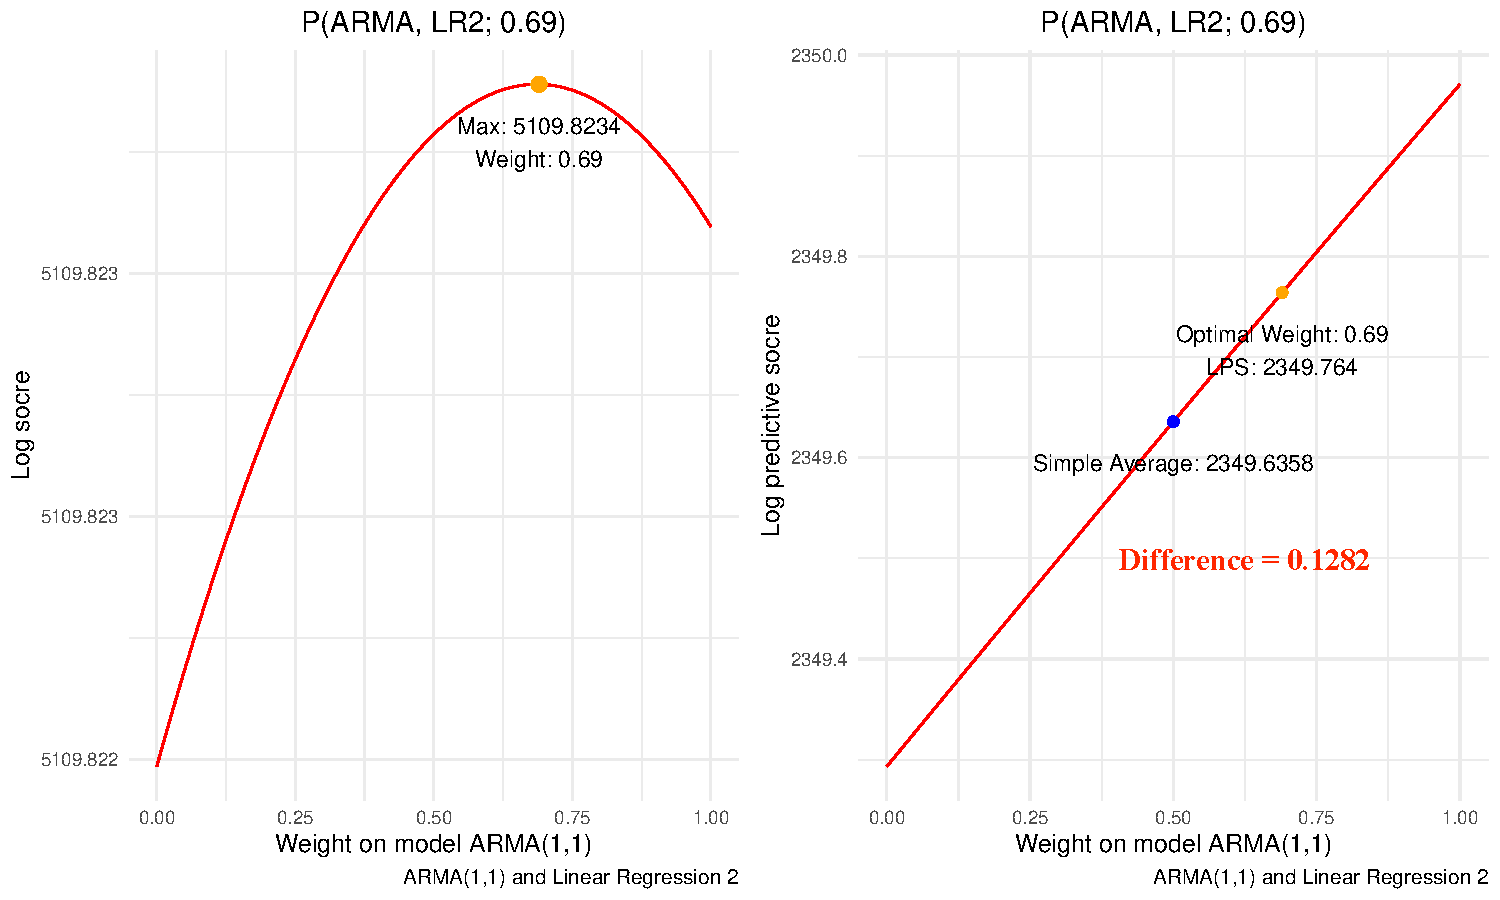
\includegraphics[scale=0.6]{figures/SP500_stationary.pdf}
\caption{Log predictive score of S\&P 500 log returns predictive densities in two-model pools over the in-sample (left) and the out-of-sample (right) period. The x-axis represents the weight assigned on the ARMA(1,1) model and the y-axis indicates the log predictive score. The meanings of colored dots remain the same as before.}
\label{fig:stat}
\end{figure}

\begin{table}[ht]
  \centering
    \begin{tabular}{l|ccc}
    \toprule
                                    &     P(ARMA,LR2;0.69)    \\  
    \midrule
    First Model Log Likelihood      &         5109.8071       \\
    Second Model Log Likelihood     &         5109.8054       \\
    Log Likelihood Difference       &          0.0016         \\
    Type                            &          (G,G)          \\
    Presence of the puzzle          &           Yes           \\
    \bottomrule
    \end{tabular}
  \caption{``Log Likelihood Difference`` represents the absolute difference of in-sample fit between two models, which is evaluated by the log likelihood. ``Type`` refers to the case of two models in the conjecture table. ``Presence of the puzzle`` indicates whether the simple average is close to or outperforms the optimal forecast combination.}
  \label{tab:statfit}
\end{table}

This Section \ref{sp500} provides some empirical evidence for our initial conjecture. When both models fit the data well, i.e., they are \texttt{Good} models, then the accuracy of the optimal density forecast combination is close to that of the average density forecast, indicating the presence of the forecast combination puzzle. If one model is \texttt{Bad} and the other is \texttt{Good}, then, at least, the puzzle can be evidenced.

\hypertarget{seasonal-time-series}{%
\section{Seasonal time series}\label{seasonal-time-series}}

With the purpose of further examining our conjecture as to when the puzzle will be in evidence, we now use a quarterly dataset to explore the relationship between the forecast combination puzzle and in-sample model fit. More specifically, we investigate cases where both models are both well-specified (good in-sample fit) or poorly-specified (poor in-sample fit). To simplify the analysis, we produce point forecasts and evaluate point combinations with MSFE.

The data considered is the recorded quarterly total number of unemployed individuals (in thousands) from 1985 Q1 to 2023 Q1, retrieved from the Australia Bureau of Statistics \autocite{ABS}. We use the natural logarithm of the total number of unemployment to reduce the level of variability in the series.

It has \(T = 153\) total observations and is slit into two sets in proportion. As before, the first 60\% of the data (\(R = 91\)), as the in-sample period, is used to estimate all unknown parameters. The remaining 40\% (\(P = 62\)) is the out-of-sample period reserved for forecast performance evaluation.

\subsection*{Well-specified models}

To ensure compatibility with seasonal component, we propose the Seasonal ARIMA (SARIMA) model and the ETS model: ARIMA(2,0,2)(0,1,1){[}4{]} with drift and ETS(A,A,A). The SARIMA is simply an ARIMA model with extra seasonal component. The first parenthesis is same as the ARIMA model. The second parenthesis represents the seasonal AR, integrated, and MA components respectively, separately by the comma. The number in the box bracket indicates the number of observations per year, i.e., the seasonal frequency. An intercept is included in the model. In the ETS model, the seasonal part is reflected by \texttt{S} and the third position in the parenthesis. Due to the log transformation, we have additive error, additive trend, and additive seasonality.

The forecast combination puzzle is evidenced in Figure \ref{fig:sd}; the accuracy difference between two combinations is negligible. The optimally-weighted point combination has a MSFE of 0.000177 and the equally-weighted forecast has a MSFE of 0.000178. Looking at the in-sample combination plot, two models fit the training set equally well, which can also be confirmed by the second column of Table \ref{tab:season}.

\begin{figure}[ht]
\centering
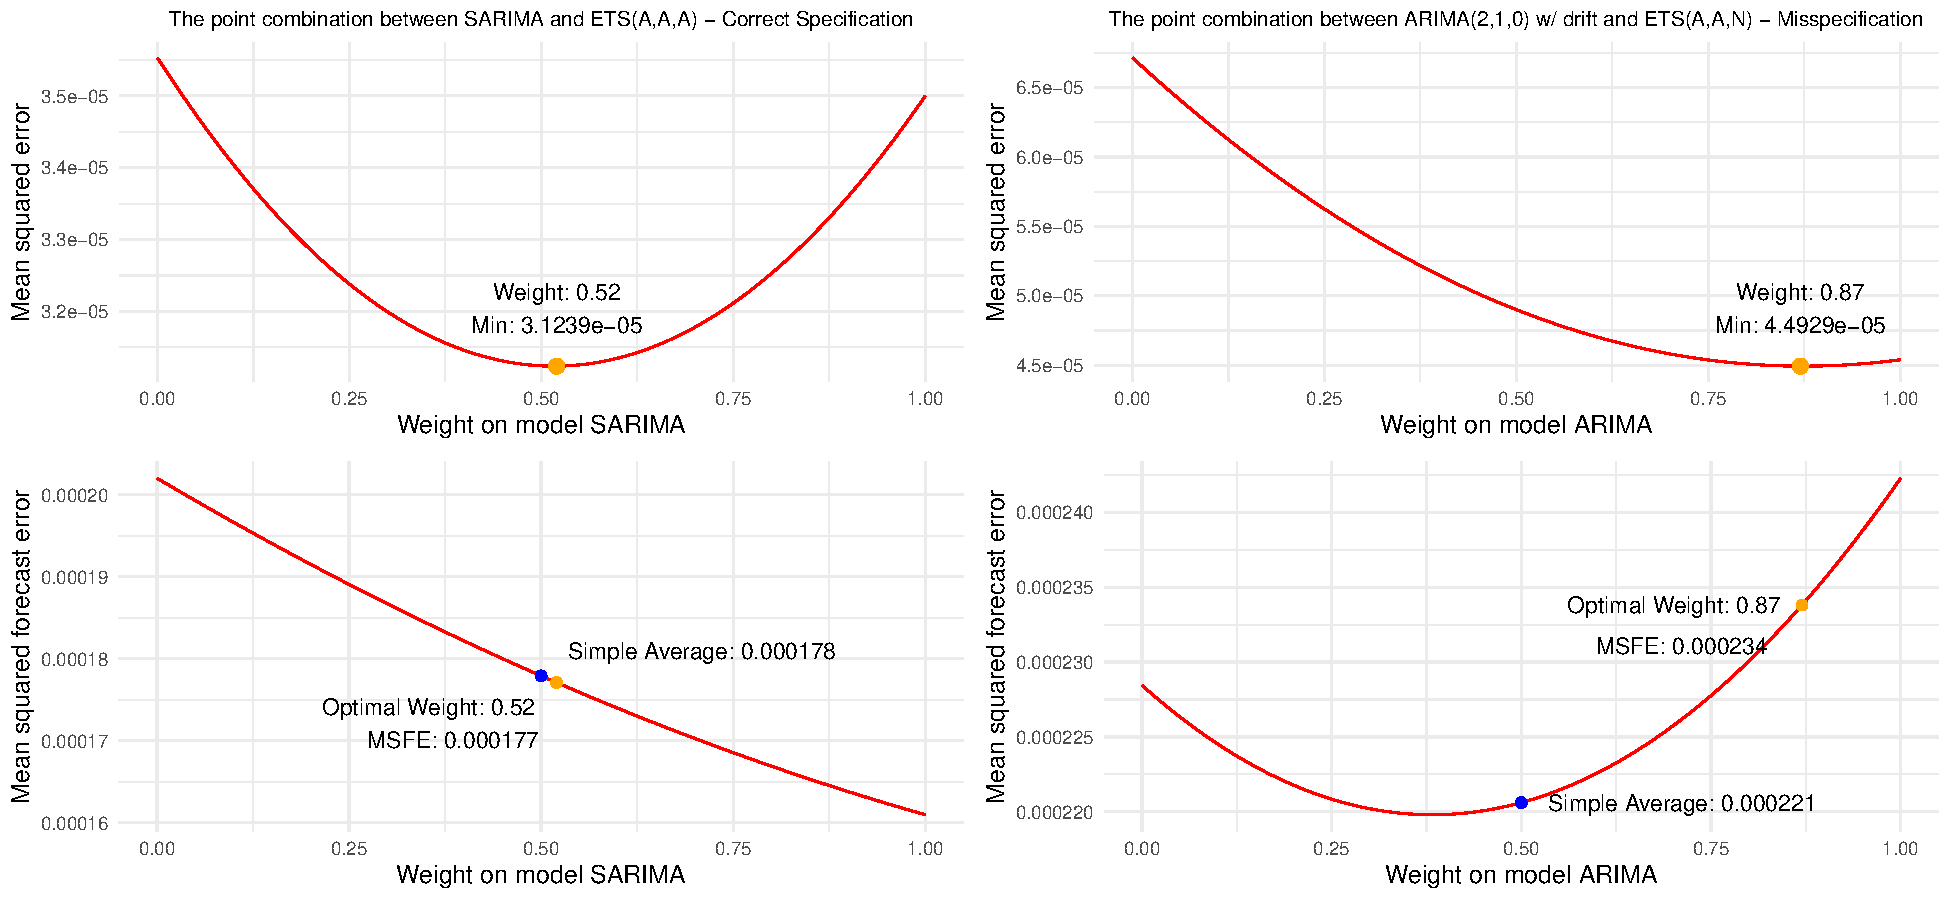
\includegraphics[scale=0.5]{figures/EMPL.pdf}
\caption{MSFE of predictive number of unemploymed people in well-specified (left) and pooly-specified (right) two-model pools over the in-sample (top) and out-of-sample (bottom) period. The x-axis represents the weight assigned on the first model and the y-axis indicates the value of MSFE. The meanings of colored dots remain the same.}
\label{fig:sd}
\end{figure}

\subsection*{Poorly-specified models}

One way of proposing a \texttt{Bad} model for a seasonal dataset is to deliberately ignore the seasonality in data. In this section, we consider the ARIMA(2,1,0) and ETS(A,A,N) models, which do not capture any seasonal component and are the best models automatically selected by \texttt{ARIMA} and \texttt{ETS} functions in R.

\begin{table}[ht]
  \centering
    \begin{tabular}{l|ccc}
    \toprule
                                      &   P(SARIMA,ETS;0.52)   &   P(ARIMA,ETS;0.87)  \\  
    \midrule
    First Model Log Likelihood        &         321.4497       &      322.1642        \\
    Second Model Log Likelihood       &         260.9102       &      231.9507        \\
    Log Likelihood Difference         &         60.5395        &      90.2135         \\
    Type                              &          (G,G)         &       (B,B)          \\
    Presence of the puzzle            &           Yes          &        Yes           \\
    \bottomrule
    \end{tabular}
  \caption{``Log Likelihood Difference`` represents the absolute difference of in-sample fit between two models, which is evaluated by the log likelihood. ``Type`` refers to the case of two models in the conjecture table. ``Presence of the puzzle`` indicates whether the simple average is close to or outperforms the optimal forecast combination.}
  \label{tab:season}
\end{table}

The right column of Figure \ref{fig:sd} does reveal the forecast combination puzzle, as the equally-weighted combination performs better than the optimally-weighted forecast combination. Furthermore, the third column of Table \ref{tab:season} illustrates that both models have similar log likelihood. We may claim that, regardless of whether the constituent models capture all the features of the data, as long as they have similar in-sample performance, the forecast combination puzzle will be evidenced. As a result, we should also expect to find the puzzle if two models are equally \texttt{Bad}.

The empirical evidence suggest that the puzzle is in evidence in all cases, however, these examples are not enough to draw comprehensive conclusions. Also, one big challenge of working with empirical data is that the true DGP is unknown.

To partially circumvent these issues, we use a simulation experiment based on a pure cross-sectional process to further investigate when the optimal forecast combination is more accurate than the simple averaging. Compared with simulated time series data, there is no need to consider the dependence of observations, hence, is an easy starting point. As an additional contribution, it examines the presence of the forecast combination puzzle in the cross-sectional setting.

\hypertarget{pure-cross-sectional-analysis}{%
\chapter{Pure Cross-sectional Analysis}\label{pure-cross-sectional-analysis}}

Given that forecast combinations can greatly improve forecast accuracy, this idea can also be applied to the pure cross-sectional settings. Remark that the use of prediction combinations is not common in such setting. In this section, we derive an analytical closed-form expression of the optimal weight under mean squared forecast error to investigate the determinants behind the puzzle in the cross-sectional setting. A simulation study is then conducted to evaluate and verify the applicability of findings.

Compared with real-life data, implementing simulation is easy to control and interpret given that the true DGP is known. Meanwhile, it is an effective way of validating our conjecture by freely changing the elements of true DGP and looking for the forecast combination puzzle. In line with previous notations, but in the cross-sectional setting, the subscript \texttt{t} will change to \texttt{i} to represent each individual observation.

\hypertarget{model-setup}{%
\section{Model Setup}\label{model-setup}}

The true DGP is assumed to be a linear regression model with no intercept and only two exogenous and weakly correlated regressors, which satisfy all assumptions of the classical linear regression model:
\begin{equation}
\label{eqn:DGP}
y_i = \beta_1 x_{1i} + \beta_2 x_{2i} + \epsilon_i, \ \ \epsilon_i \stackrel{i.i.d}{\sim} N(0,\sigma^2_{\epsilon}) \ \ \ (i = 1,2,...,N). \\
\end{equation}

The forecasting models, or constituent models, are
\begin{align*}
M_1: y_i &= \alpha_1 x_{1i} + e_{1i}, \ \ e_{1i} \stackrel{i.i.d}{\sim} N(0,\sigma^2_1) \\
M_2: y_i &= \alpha_2 x_{2i} + e_{2i}, \ \ e_{2i} \stackrel{i.i.d}{\sim} N(0,\sigma^2_2).
\end{align*}

\hypertarget{op}{%
\section{Optimal Weight (MSE)}\label{op}}

Following the methodology in Section \ref{method}, the observed data are divided into an in-sample period (\(R\)) for parameter estimation and an out-of-sample period (\(P\)) for accuracy evaluation. As noted before, the estimated optimal weight, \(\hat\omega_{opt}\), will be generated using the first R number of observations, and held fixed over the P observation.

To simplify the notation, we use the notation for linear regression models in matrix form, and obtain the following formula for \(\hat\omega_{opt}\) under the MSE loss
\begin{equation*}
\hat\omega_{opt} = \frac{(x_1 \hat\alpha_1 - x_2 \hat\alpha_2)' y - (x_1 \hat\alpha_1 - x_2 \hat\alpha_2)' x_2 \hat\alpha_2}{\hat\alpha'_1 x'_1 x_1 \hat\alpha_1 - 2\hat\alpha'_1 x'_1 x_2 \hat\alpha_2 + \hat\alpha'_2 x'_2 x_2 \hat\alpha_2},
\end{equation*}
where \(\hat\alpha_1\) and \(\hat\alpha_2\) are the ordinary least squares estimators in \(M_1\) and \(M_2\) respectively.

A more meaningful expression can be achieved by multiplying \(\frac{1}{R}\) to both numerator and denominator and writing
\begin{equation*}
\label{eqn:opt}
\hat\omega_{opt} = \frac{\hat\alpha_1'\text{cov}_R(x_1,x_1)\hat\alpha_1 - \hat\alpha_1'\text{cov}_R(x_1,x_2)\hat\alpha_2}{\hat\alpha_1' \text{cov}_R(x_1,x_1)\hat\alpha_1 - 2\hat\alpha_1'\text{cov}_R(x_1,x_2)\hat\alpha_2 + \hat\alpha_2'\text{cov}_R(x_2,x_2)\hat\alpha_2},
\end{equation*}
where \(\text{cov}_R(x_j,x_k)\) is the in-sample covariance between regressors \(x_j\) and \(x_k\).

In the classical linear regression setting, OLS estimator is consistent when the sample size goes to infinity. That is, we should have \(\hat\alpha_1 \overset{p}{\to} \alpha_1\) and \(\hat\alpha_2 \overset{p}{\to} \alpha_2\). Considering the limit result, we have
\begin{equation}
\label{eqn:limit}
\hat\omega_{opt} \overset{p}{\to} \omega_\star = \frac{\alpha_1'\Sigma_{11}\alpha_1 - \alpha_1'\Sigma_{12}\alpha_2}{\alpha_1'\Sigma_{11}\alpha_1 - 2\alpha_1'\Sigma_{12}\alpha_2 + \alpha_2'\Sigma_{22}\alpha_2},
\end{equation}
where \(\omega_\star\) is the limiting value of the optimal weight, \(\Sigma_{jk}\) denotes the population covariance matrix of corresponding regressors \(x_j\) and \(x_k\). With the limit result in equation (\ref{eqn:limit}), we can easily work out the asymptotic determinants of having \(\omega_\star=\frac{1}{2}\) and then connect it with the presence of the puzzle.

For \(\omega_\star=\frac{1}{2}\), it must be that \(\alpha_1'\Sigma_{11}\alpha_1 = \alpha_2'\Sigma_{22}\alpha_2\), which suggests a symmetrical relationship between two constituent model. This gives rigorous evidence that similar in-sample performance of two models will lead to the presence of the puzzle. Besides, any situation where this final equality is nearly satisfied will inevitably lead an optimal weight near one-half.

In addition, according to the relationship between \(\pmb \alpha\) and \(\pmb \beta\) in Appendix \ref{detail}, \(\alpha_1\) and \(\alpha_2\) will be close to \(\beta_1\) and \(\beta_2\), respectively, when the correlation between regressors is small. This suggests that the optimal weight interacts with the true data generating process and is therefore related to the true DGP.

\begin{figure}[ht]
\centering
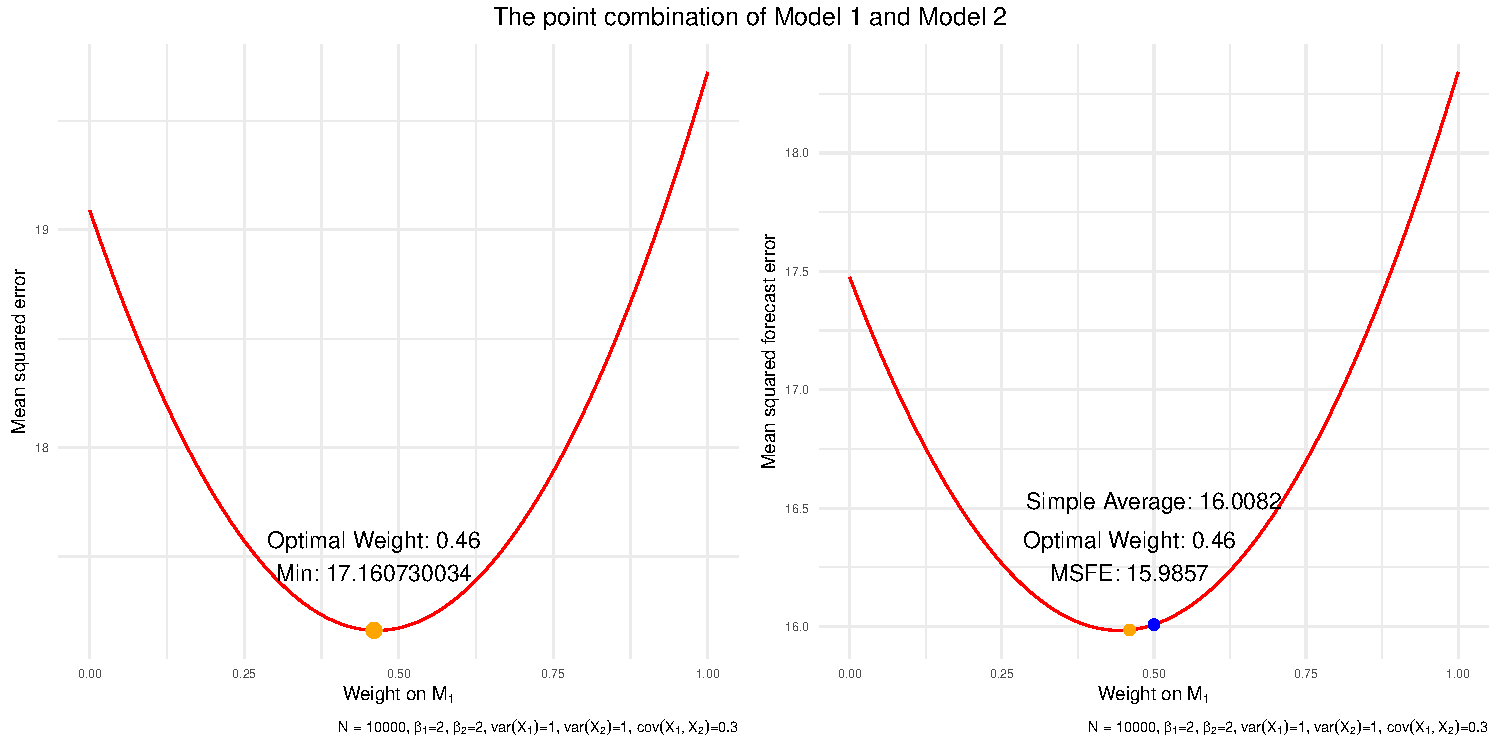
\includegraphics[scale=0.6]{figures/MSFE.pdf}
\caption{MSFE of predictive points in a two-model pool over the in-sample (left) and the out-of-sample (right) period. The x-axis represents the weight assigned on $M_1$ and the y-axis indicates MSFE. The orange dot represents the optimally-weighted combination, while the blue dot indicates the equally-weighted combination.}
\label{fig:msfe}
\end{figure}

Figure \ref{fig:msfe} illustrates one example of having \(\hat\omega_{opt}\) equal to 0.5 when \(N = 10000\), \(\beta_1=\beta_2=2\), \(Var(X_1)=Var(X_2)=1\), \(Cov(X_1,X_2)=0.3\) under the MSE weighting scheme. Both in-sample and out-of-sample curves look symmetric.

\hypertarget{density-simulations}{%
\section{Density Simulations}\label{density-simulations}}

Recall the equation (\ref{eqn:LS2}) in Section \ref{method}, it is clear that the weight \(\omega\) appears in the natural logarithm function. The expectation operator can only evaluate the first derivative of equation (\ref{eqn:LS2}) with respect to \(\omega\) by integration. As a consequence, there is no closed-form limiting expression for the optimal weight \(\hat\omega_{opt}\) under log score. However, we can use a simulation study to examine the applicability of findings from Section \ref{op} to density combinations and log scoring rules.

The initial set-up has 10000 (N) artificial cross-sectional observations generated from the equation (\ref{eqn:DGP}) with \(E[X_{1i}] = E[X_{2i}] = 0\), \(Var(X_{1i}) = Var(X_{2i}) = 1\), \(Cov(X_{1i}, X_{2i}) = 0.3\), \(\pmb{\beta} = (\beta_1, \beta_2)' = (2,2)'\), and \(\sigma^2_{\epsilon}=4\). Same as before, around 60\% of the data will be used for model estimation. The density forecast combinations will follow the construction of two-model pools and be evaluated using the log score.

\begin{figure}[ht]
\centering
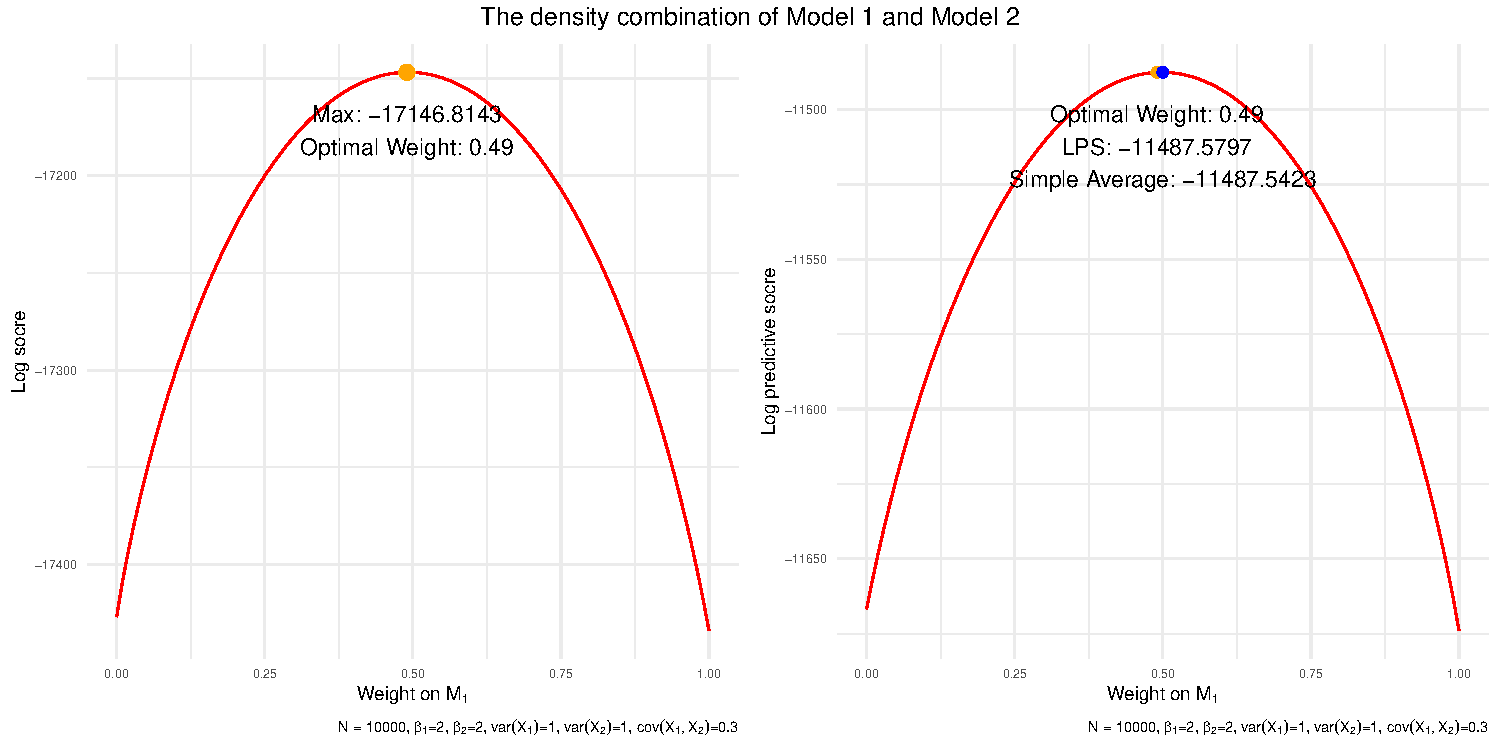
\includegraphics[scale=0.6]{figures/LPS_10000.pdf}
\caption{Two curves refer to the in-sample (left) and out-of-sample (right) performance of density combinations with artificial cross-sectional data based on the initial set-up. The x-axis represents the weight assigned on $M_1$ and the y-axis indicates the log score. The meanings of colored dots remain unchanged.}
\label{fig:ss10000}
\end{figure}

\begin{figure}[ht]
\centering
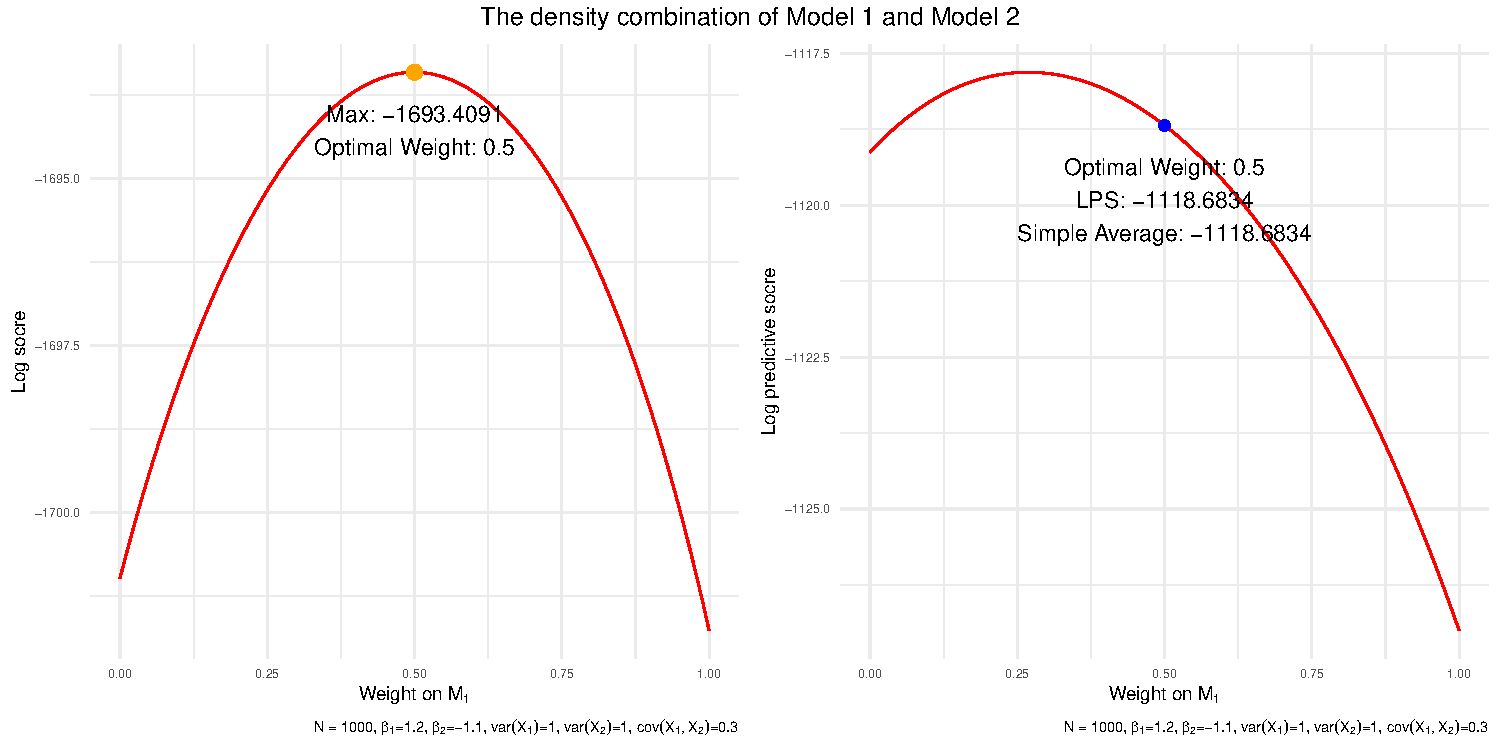
\includegraphics[scale=0.6]{figures/LPS_1000.pdf}
\caption{Two curves refer to the in-sample (left) and out-of-sample (right) performance of density combinations with artificial cross-sectional data. The x-axis represents the weight assigned on $M_1$ and the y-axis indicates the log score. The meanings of dots remain unchanged.}
\label{fig:ss1000}
\end{figure}

Using the same model specification as in Figure \ref{fig:msfe} to construct the density forecast combination via the log score, we see that the optimal weight \(\hat\omega_{opt}\) is no longer one-half in Figure \ref{fig:ss10000}. On the other hand, Figure \ref{fig:ss1000} shows that \(\hat\omega_{opt}\) is equal to one-half when \(N = 1000\), \(\beta_1=1.2\), \(\beta_2=-1.1\). This indicates that besides the magnitude of \(\pmb{\beta}\), the sign will also have an impact on \(\hat\omega_{opt}\), even in large samples (\(N = 50000\)). Therefore, we speculate that the optimal weight has a non-linear relationship with the proposed models under the log score weighting scheme.

\begin{figure}[ht]
\centering
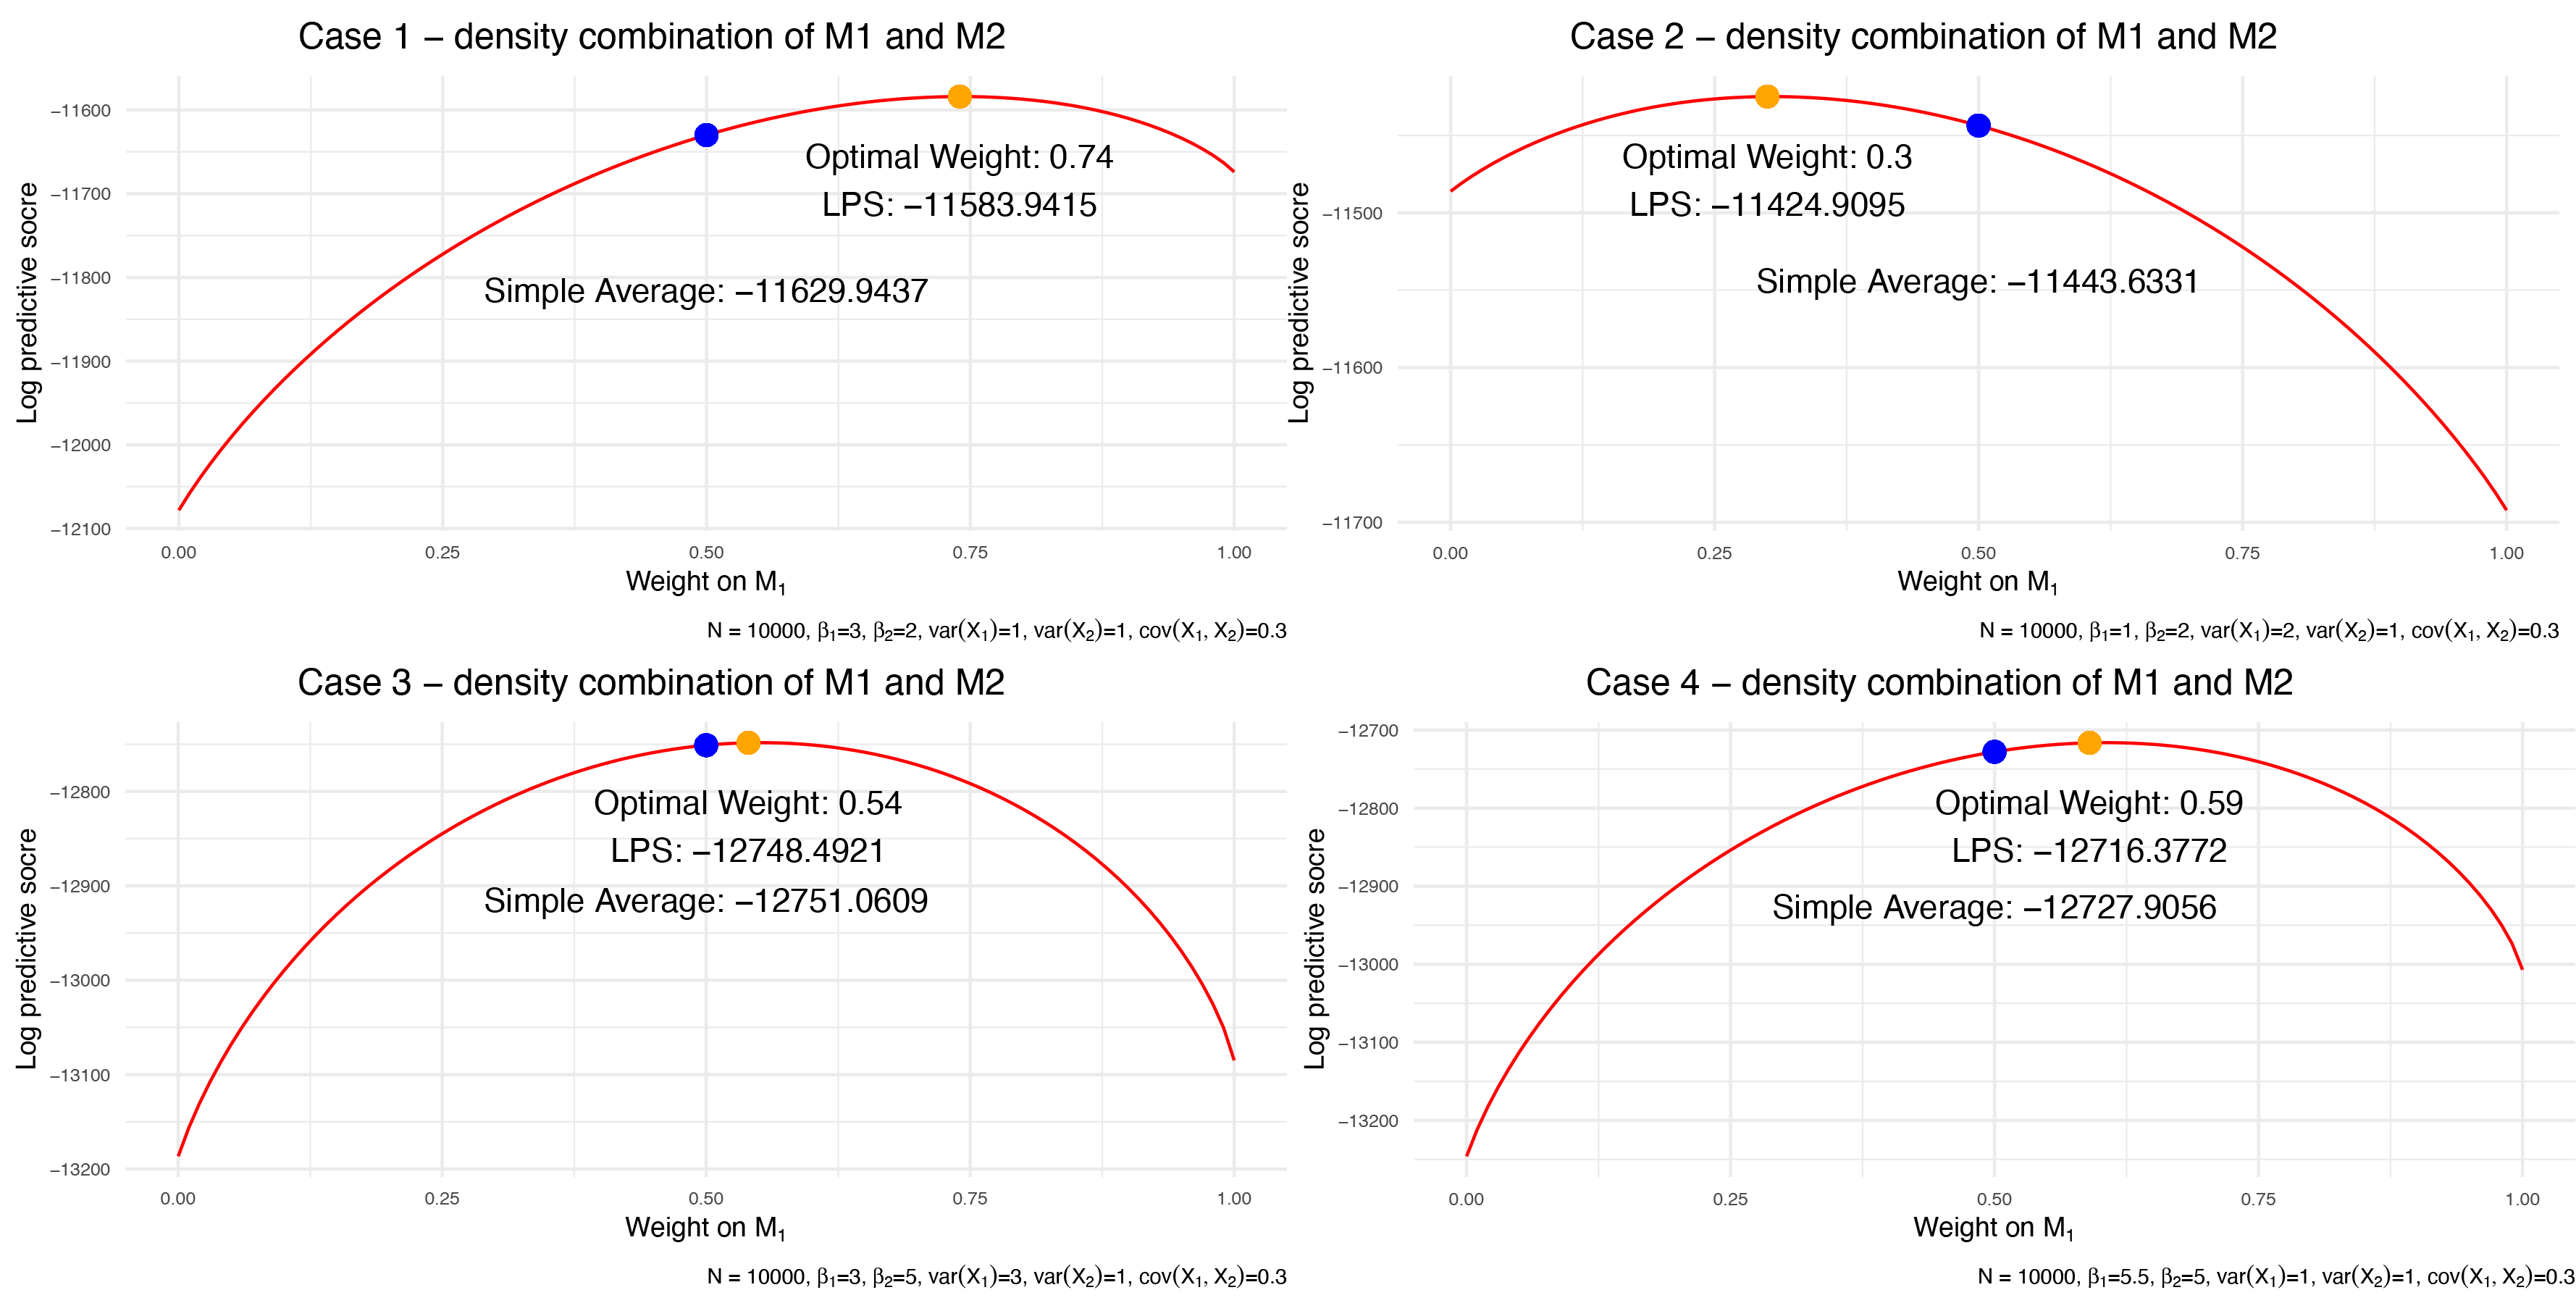
\includegraphics[scale=0.53]{figures/con_cases.png}
\caption{The out-of-sample performance of density combinations with artificial cross-sectional data. The true DGP are in the bottom-right of individual plots. ``Optimal Weight`` shows the estimated optimal weight. The log predictive scores of optimally-weighted combination and equally-weighted combination are indicated by ``LPS`` and ``Simple Average`` respectively.}
\label{fig:cases}
\end{figure}

In the regression setting, we evaluate the in-sample performance with \(R^2\), and then link this value to the conjecture in Table \ref{tab:1}. Four cases in Figure \ref{fig:cases} are selected to further validate different types of model combinations as empirical evidence. Clearly, the optimally-weighted combination outperforms the equally-weighted combination with higher forecast accuracy in the first two cases; hence, we do not have the forecast combination puzzle. After comparing the in-sample fit of constituent models with \(R^2\), these two pools can be labelled as (G,B) and (B,G), respectively, as summarized in Table \ref{tab:cases}. This supports our preliminary conjecture that when two models have differing levels of in-sample performance, the presence of the puzzle is unclear, i.e., the puzzle may or may not occur.

\begin{table}[ht]
  \centering
    \begin{tabular}{l|cccc}
    \toprule
                              &    Case 1    &    Case 2   &    Case 3    &    Case 4   \\  
    \midrule
    $R^2$ of $M_1$            &    0.393     &    0.141    &    0.476     &    0.558    \\
    $R^2$ of $M_2$            &    0.256     &    0.224    &    0.452     &    0.504    \\
    $R^2$ Difference          &    0.138     &    0.083    &    0.024     &    0.053    \\
    Type                      &    (G,B)     &    (B,G)    &    (B,B)     &    (G,B)    \\
    Presence of the puzzle    &     No       &     No      &     Yes      &     No     \\
    \bottomrule
    \end{tabular}
    \caption{``Difference`` is the absolute difference of in-sample $R^2$ between two models. ``Type`` refers to the case of two models in the conjecture table. ``Presence of the puzzle`` indicates whether the equally-weighted combination is close to or outperforms the optimally-weighted combination.}
  \label{tab:cases}
\end{table}

Recall that in our definition of the forecast combination puzzle, small accuracy differences make it hard to decide whether the puzzle is in evidence. For example, cases 3 and 4 in Figure \ref{fig:cases} both illustrate a close distance between the optimal forecast combination and the simple average. Even the \(R^2\) of constituent models in each pool are similar, as indicated by Table \ref{tab:cases}. One possible solution is to formally test the statistical significance of the accuracy difference through the Diebold-Mariano Test \autocite{D15}. Unfortunately, it has been proven that the test is not appropriate in this context as the test statistic will not follow a standard normal distribution using the two-stage estimation \autocite{FZMP23}. Another possible choice is deciding on an arbitrary value for the accuracy difference. It turns out that the magnitude of the log predictive score is tightly related to the sample size and assumptions about the error term in the true DGP. Hence, this method can be used when fixing the sample size and assumptions of the error term.

Instead of forecast accuracy, we can look at the difference in in-sample \(R^2\). One possible rule of thumb is that when the absolute difference of in-sample \(R^2\) between two models is less than 0.05, i.e., two models have similar in-sample fit, then the two-model pool can be viewed as either the (G,G) or (B,B) case, and therefore the puzzle seems to be in evidence. Applying this finding to cases 3 and 4 in Table \ref{tab:cases}, case 3 is a (G,G) case where its in-sample \(R^2\) difference is 0.024, less than 0.05, whereas case 4 is a (G,B) case with a 0.053 in-sample \(R^2\) difference, slightly higher than 0.05. By using this rule of thumb, we can only be certain that the puzzle is evident in case 3 but we are unconfident in case 4. In terms of the log likelihood, it is highly affected by the sample size, similar to the log predictive score. One possible way, however, is to normalize the difference of two log likelihoods by their sum based on the chosen constituent models. The heuristic is around 0.009, meaning that when the normalized difference is less than 0.009, two models have similar in-sample fit, and therefore the puzzle is likely to be in evidence.

\begin{table}[ht]
\centering
\begin{tabular}{cccc}
                       &      & \multicolumn{2}{c}{$M_2$} \\
                       &      & Good       & Bad       \\
\multirow{2}{*}{$M_1$} & Good & $\surd$    & $?$ \\
                       & Bad  & $?$        & $\surd$
\end{tabular}
\caption{The first row and the first column refer to two constituent models, $M_1$ and $M_2$. ``Good`` and ``Bad`` denote the relative in-sample fit of constituent model. The ``$\surd$`` indicates the presence of the forecast combination puzzle, while ``$?$`` implies that the presence of the puzzle is ambiguous.}
\label{tab:2}
\end{table}

The analysis in this section provides a general idea of the relationship between the in-sample fit of constituent models and the presence of the puzzle in both point and density forecast combinations. Based on new empirical evidence, the conjecture table for a two-model pool remains the same but with updated definitions, as illustrated in Table \ref{tab:2}.

\hypertarget{conclusion}{%
\chapter{Conclusion}\label{conclusion}}

This thesis develops a means of determining the presence of the forecast combination puzzle in a two-model pool by closely examing in-sample model fit. Empirical results suggest that when both constituent models have similar in-sample fit, poor or good, the equally-weighted combination will provide equivalent forecast accuracy relative to the optimally-weighted combination. On the other hand, when the in-sample fit differs between the two models, the presence of the puzzle is ambiguous.

Importantly, in a linear regression context, we derive the relationship between the optimal weight and elements in the proposed models under mean squared error scheme when using point combinations. According to the closed-form expression for the estimated optimal weight, the presence of the puzzle is tightly-related to the sample size, the sign and magnitude of parameters in the constituent models, the sample variances of regressors, and the correlation between regressors. It is also shown that a large difference in the in-sample performance of proposed models can move the estimated optimal weight away from one-half (equal weights), especially in large samples. Additionally, the optimal weight also interacts with the true DGP in a broad sense, which determines the estimated coefficients in the constituent models.

Not surprisingly, these findings can be applied to density combinations under log predictive score, where the estimated optimal weight does not have a closed-form expression. While the two constituent models have a symmetrical relationship when the population weight is equal to one-half in the MSE case, we find empirical evidence that this may not be the same case under log score.

Working with the two-model pools provides an opportunity to explore a variety of situations in a short period of time. The next natural step is to investigate multiple forecast combinations. It is also necessary to relax some of the restrict model assumptions and increase the complexity of the model structure in our simulation study. Under the explicit definition of the forecast combination puzzle, it is hard to determine the significance of the accuracy difference between optimally-weighted combination and equally-weighted combination, given that neither the testing or an arbitrary choice will work for all cases. We leave these, and other interesting issues, for future research.

\appendix

\hypertarget{appendix}{%
\chapter{Appendix}\label{appendix}}

All codes are performed in R Statistical Software (version 4.2.1 (2022-06-23)). The packages used are \texttt{tidyverse} \autocite{tidy19}, \texttt{dplyr} \autocite{dplyr23}, \texttt{fpp3} \autocite{fpp23}, \texttt{gridExtra} \autocite{gridExtra}, and \texttt{mvtnorm} \autocite{GBMMLSH21}. Full code and data are available online in GitHub repository: \url{https://github.com/Sapphire-Li/Honours_Research_Project}.

\hypertarget{model-specification}{%
\section{Model Specification}\label{model-specification}}

The error term, \(\epsilon_t\), in each model is assumed to be independent and normally distributed with a zero mean and a constant variance. Each model is independent. Even if using the same notation for unknown parameters across models, the estimators are different. The index \(t\) takes the values from \(1\) to the total sample size \(T\).

Exact formulas and explanations of these models can be found in \textcite{fpp3}. The formula of the conditional variance for the ETS(M,N,N) model is discussed in Chapter 6.3 of \textcite{HKOS08}.

\hypertarget{nonstationary-sp-500-index}{%
\subsection{Nonstationary S\&P 500 Index}\label{nonstationary-sp-500-index}}

\begin{enumerate}
\def\labelenumi{\arabic{enumi}.}
\item
  ARIMA(1,1,1) model with an intercept of the natural logarithm of S\&P 500 index.
  \begin{equation*}
  log(y_t) = c + log(y_{t-1}) + \phi_1\big[log(y_{t-1})-log(y_{t-2})\big] + \epsilon_t + \theta_1\epsilon_{t-1}
  \end{equation*}
\item
  ETS(M,N,N) model of the natural logarithm of S\&P 500 index.
  \begin{align*}
  log(y_t) &= \ell_{t-1} (1+\epsilon_t) \\
  \ell_t &= \ell_{t-1} (1+\alpha \epsilon_t) \\
  \end{align*}
\item
  A classical linear regression model of the natural logarithm of the S\&P 500 index and ARIMA(1,0,0) errors.
  \begin{align*}
  log(y_t) &= \beta_0 + \beta_1 t + u_t \\
  u_t &= \phi_1 u_{t-1} + \epsilon_t
  \end{align*}
\end{enumerate}

\hypertarget{stationary-sp-500-index}{%
\subsection{Stationary S\&P 500 Index}\label{stationary-sp-500-index}}

\begin{enumerate}
\def\labelenumi{\arabic{enumi}.}
\item
  ARMA(1,1) model with an intercept of the natural logarithm of S\&P 500 returns.
  \begin{equation*}
  log(y_t) - log(y_{t-1}) = c + \phi_1\big[log(y_{t-1})-log(y_{t-2})\big] + \epsilon_t + \theta_1\epsilon_{t-1}
  \end{equation*}
\item
  A classical linear regression model of the natural logarithm of the S\&P 500 returns and ARMA(1,1) errors.
  \begin{align*}
  log(y_t) - log(y_{t-1}) &= \beta_0 + u_t \\
  u_t &= \phi_1 u_{t-1} + \epsilon_t + \theta_1\epsilon_{t-1}
  \end{align*}
\end{enumerate}

\hypertarget{well-specified-models-for-seasonal-unemployment-dataset}{%
\subsection{Well-specified Models for Seasonal Unemployment Dataset}\label{well-specified-models-for-seasonal-unemployment-dataset}}

\begin{enumerate}
\def\labelenumi{\arabic{enumi}.}
\item
  ARIMA(2,0,2)(0,1,1){[}4{]} model with an intercept of the natural logarithm of unemployed individuals.
  \begin{align*}
  log(y_t) &= c + log(y_{t-4}) + \phi_1\big[log(y_{t-1})-log(y_{t-5})\big] + \phi_2\big[log(y_{t-2})-log(y_{t-6})\big] \\
        &+ \epsilon_t + \theta_1\epsilon_{t-1} + \theta_2\epsilon_{t-2} + \Theta_1\epsilon_{t-4} + \theta_1\Theta_1\epsilon_{t-5} + \theta_2\Theta_1\epsilon_{t-6} \\
  \end{align*}
\item
  ETS(A,A,A) model of the natural logarithm of unemployed individuals.
  \begin{align*}
  log(y_t) &= \ell_{t-1} + b_{t-1} + s_{t-m} + \epsilon_t \\
  \ell_t &= \ell_{t-1} + b_{t-1} + \alpha \epsilon_t \\
  b_t &= b_{t-1} + \beta \epsilon_t \\
  s_{t} &= s_{t-m} + \gamma \epsilon_t
  \end{align*}
\end{enumerate}

\hypertarget{poorly-specified-models-for-seasonal-unemployment-dataset}{%
\subsection{Poorly-specified Models for Seasonal Unemployment Dataset}\label{poorly-specified-models-for-seasonal-unemployment-dataset}}

\begin{enumerate}
\def\labelenumi{\arabic{enumi}.}
\item
  ARIMA(2,1,0) model with an intercept of the natural logarithm of unemployed individuals.
  \begin{equation*}
  log(y_t) = c + log(y_{t-1}) + \phi_1\big[log(y_{t-1})-log(y_{t-2})\big] + \phi_2\big[log(y_{t-2})-log(y_{t-3})\big] + \epsilon_t
  \end{equation*}
\item
  ETS(A,A,N) model of the natural logarithm of unemployed individuals.
  \begin{align*}
  log(y_t) &= \ell_{t-1} + b_{t-1} + \epsilon_t \\
  \ell_t &= \ell_{t-1} + b_{t-1} + \alpha \epsilon_t \\
  b_t &= b_{t-1} + \beta \epsilon_t
  \end{align*}
\end{enumerate}

\hypertarget{detail}{%
\section{Optimal Weight Derivation Details}\label{detail}}

In this section, we detail the derivation steps of producing the results in Section \ref{op}.

Recall that the data is drawn from the true DGP:
\[y_i = \beta_1 x_{1i} + \beta_2 x_{2i} + \epsilon_i, \ \ \epsilon_i \stackrel{i.i.d}{\sim} N(0,\sigma^2_{\epsilon}) \ \ \ (i = 1,2,...,N),\]
where the in-sample period (R) is used to estimate the parameters for the following two constituent models:
\begin{align*}
M_1: y_i &= \alpha_1 x_{1i} + u_{1i}, \ \ u_{1i} \stackrel{i.i.d}{\sim} N(0,\sigma^2_1) \\
M_2: y_i &= \alpha_2 x_{2i} + u_{2i}, \ \ u_{2i} \stackrel{i.i.d}{\sim} N(0,\sigma^2_2).
\end{align*}

Besides, we allow \(x_{1i}\) and \(x_{2i}\) to have a small correlation, otherwise, there may be multicollinearity, resulting in higher standard errors of estimated parameters.

For simplicity, these models can be written in matrix form
\begin{align*}
y &= x_1 \beta_{1} + x_2 \beta_{2} + \epsilon, \\
M_1 : y &= x_1 \alpha_{1} + u_1, \\
M_2 : y &= x_2 \alpha_{2} + u_2,
\end{align*}
where
\[
     {y}=\begin{bmatrix}
           y_{1} \\
           y_{2} \\
           \vdots \\
           y_{N}
         \end{bmatrix},\;
     {x_1}=\begin{bmatrix}
           x_{11} \\
           x_{21} \\
           \vdots \\
           x_{N1}
         \end{bmatrix},\;
    {x_2}=\begin{bmatrix}
           x_{12} \\
           x_{22} \\
           \vdots \\
           x_{N2}
         \end{bmatrix},\;
    {\epsilon}=\begin{bmatrix}
           \epsilon_{1} \\
           \epsilon_{2} \\
           \vdots \\
           \epsilon_{N}
         \end{bmatrix}.
\]

Applying the OLS estimation, we can immediately obtain the formula of \(\hat\alpha_{1}\) and \(\hat\alpha_{2}\). Given a weak correlation between regressors, each formula will have an extra component, which represents that correlation.
\begin{align*}
    \hat\alpha_{1} &= (x'_1x_1)^{-1} x'_1y \\
    &= (x'_1x_1)^{-1} x'_1(x_1 \beta_1 + x_2 \beta_2 + \epsilon) \\
    &= \beta_1 + (x'_1x_1)^{-1} x'_1x_2 \beta_2 \\
    &= \beta_1 + var(x_1)^{-1} cov(x_1,x_2) \beta_2 \\
    \\
    \hat\alpha_{2} &= (x'_2x_2)^{-1} x'_2y \\
    &= (x'_2x_2)^{-1} x'_2(x_1 \beta_1 + x_2 \beta_2 + \epsilon) \\
    &= \beta_2 + (x'_2x_2)^{-1} x'_2x_1 \beta_1 \\
    &= \beta_2 + var(x_2)^{-1} cov(x_2,x_1) \beta_1 \\
\end{align*}
\begin{align*}
    \hat y_{\omega} &= \hat y_1 \omega + \hat y_2 (1-\omega) \\
    &= x_1 \hat\alpha_1 \omega + \ x_2 \hat\alpha_2 (1-\omega) \\
    &= x_1 \hat\alpha_1 \omega - x_2 \hat\alpha_2 \omega + x_2 \hat\alpha_2 \\
    &= (x_1 \hat\alpha_1 - x_2 \hat\alpha_2) \omega + x_2 \hat\alpha_2 
\end{align*}

\begin{align*}
\hat{\omega}_{\text{opt}} 
&= \underset{\omega \in [0,1]}{\arg\min} \ \frac{1}{R} \big(y - \hat y_{\omega}\big)' \big(y - \hat y_{\omega}\big) \\
&= \underset{\omega \in [0,1]}{\arg\min} \ \frac{1}{R} \big[y-(x_1 \hat\alpha_1 - x_2 \hat\alpha_2) \omega - x_2 \hat\alpha_2\big]'\big[y-(x_1 \hat\alpha_1 - x_2 \hat\alpha_2) \omega - x_2 \hat\alpha_2\big]
\end{align*}
\begin{align*}
    -2(x_1 \hat\alpha_1 - x_2 \hat\alpha_2)' (y-(x_1 \hat\alpha_1 - x_2 \hat\alpha_2) \hat\omega_{opt} - x_2 \hat\alpha_2) &= 0 \\
    (x_1 \hat\alpha_1 - x_2 \hat\alpha_2)' (x_1 \hat\alpha_1 - x_2 \hat\alpha_2) \hat\omega_{opt} &= (x_1 \hat\alpha_1 - x_2 \hat\alpha_2)' (y - x_2 \hat\alpha_2) \\
    \hat\omega_{opt} &= \frac{(x_1 \hat\alpha_1 - x_2 \hat\alpha_2)' (y - x_2 \hat\alpha_2)}{(x_1 \hat\alpha_1 - x_2 \hat\alpha_2)' (x_1 \hat\alpha_1 - x_2 \hat\alpha_2)} \\
    \hat\omega_{opt} &= \frac{(x_1 \hat\alpha_1 - x_2 \hat\alpha_2)' (y - x_2 \hat\alpha_2)}{(x_1 \hat\alpha_1 - x_2 \hat\alpha_2)' (x_1 \hat\alpha_1 - x_2 \hat\alpha_2)} \\
    \hat\omega_{opt} &= \frac{(x_1 \hat\alpha_1 - x_2 \hat\alpha_2)' y - (x_1 \hat\alpha_1 - x_2 \hat\alpha_2)' x_2 \hat\alpha_2}{\hat\alpha'_1 x'_1 x_1 \hat\alpha_1 - 2\hat\alpha'_1 x'_1 x_2 \hat\alpha_2 + \hat\alpha'_2 x'_2 x_2 \hat\alpha_2}
\end{align*}

\hypertarget{formula-related-to-the-f-statistics}{%
\subsection{\texorpdfstring{Formula related to the \(F\)-statistics}{Formula related to the F-statistics}}\label{formula-related-to-the-f-statistics}}

To clearly see the relationship between the in-sample fit and the optimal weight, the equation (\ref{eqn:opt}) in Section \ref{op} can be linked with the F-statistics of two models. The F-test of overall significance is a formal hypothesis test, which examines the explanatory power of the whole model.

The hypothesis of the overall significance test for \(M_1\) can be written as \(H_0: R\alpha_1 = r\) and \(H_1: R\alpha_1 \ne r\) where \(R\) is a scalar 1 (or an identity matrix when \(\alpha\) is a column vector) and \(r\) is a scalar 0 (or a column vector of 0).

Define \(m\) as the number of restrictions in the null hypothesis, and the sum squared of errors (SSE) for the full (true) model \ref{eqn:DGP} is \(SSE_{full} = (y - x_1 \hat\beta_1 - x_2 \hat\beta_2)'(y - x_1 \hat\beta_1 - x_2 \hat\beta_2)\). Then the unbiased estimator of the true model variance is \(s^2=\frac{SSE_{full}}{R-2}\).

The F-statistic follows a F-distribution with degrees of freedom (1,R-2) under \(H_0\), which is defined as
\begin{align*}
F_{\alpha_1} &= (R\hat\alpha_1 - r)'[s^2R(x_1'x_1)^{-1}R']^{-1}(R\hat\alpha_1 - r)/m \\
&= (\hat\alpha_1 - 0)' \Big[s^2(x_1'x_1)^{-1}\Big]^{-1} (\hat\alpha_1 - 0)/1 \\
&= R \ s^{-2} \ \hat\alpha'_1 \text{cov}_R(x_1,x_1) \hat\alpha_1. \\
\end{align*}

Similarly, we have
\begin{equation*}
F_{\alpha_2} = R \ s^{-2} \ \hat\alpha'_2 \text{cov}_R(x_2,x_2) \hat\alpha_2 \sim F_{1,R-2} \text{ under  H}_0.
\end{equation*}

The optimal weight \(\hat\omega_{opt}\) can also be expressed with F-statistics of \(M_1\) and \(M_2\)
\begin{equation*}
\hat\omega_{opt} = \frac{F_{\alpha_1}- R \ \hat\alpha_1'\text{cov}_R(x_1,x_2)\hat\alpha_2/s^2}{F_{\alpha_1} + F_{\alpha_2} - 2 R \ \hat\alpha_1'\text{cov}_R(x_1,x_2)\hat\alpha_2/s^2}.
\end{equation*}

If the covariance between \(x_1\) and \(x_2\) is close to zero, the optimal weight can be approximated as \(\hat\omega_{opt} = \frac{F_{\alpha_1}}{F_{\alpha_1} + F_{\alpha_2}}\). This is the reason why the in-sample performance of model is highly correlated with the presence of the puzzle.

\printbibliography[title={Reference}]




\end{document}
